\section{Model-driven Development}
\begin{frame}[t]{Model-Driven Software Development (MDD)}

	\begin{columns}[T]
		\begin{column}{.48\textwidth}
			\centering
			Classic Software Development
			
			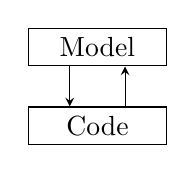
\begin{tikzpicture}[every node/.style={draw, minimum width = 50}, >=stealth]
				\node(model){Model};
				\node[below of=model](code){Code};
				\draw[->, transform canvas={xshift=-10}](model) -- (code);
				\draw[->, transform canvas={xshift= 10}](code) -- (model);
			\end{tikzpicture}
		\end{column}
		\begin{column}{.48\textwidth}
			\pause
			\centering	
			Model-driven Software Development
			
			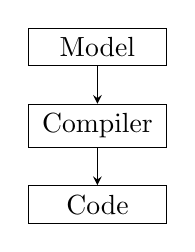
\begin{tikzpicture}[every node/.style={draw, minimum width = 50}, >=stealth]
				\node(model){Model};
				\node[below of=model](generator){Compiler};
				\node[below of=generator](code){Code};
				\draw[->](model) -- (generator);
				\draw[->](generator) -- (code);
			\end{tikzpicture}
		\end{column}
	\end{columns}
	
	\pause
	
	Advantages
	
	\begin{itemize}
		\item<+-> Better abstraction
		\item<+-> Models are easier to check for logical errors
		\item<+-> Models are easier to understand for non-programmers
	\end{itemize}
\end{frame}

\begin{frame}[t]{Model-Driven Software Development (MDD)}
	\framesubtitle{Our approch}
	
	{\centering
	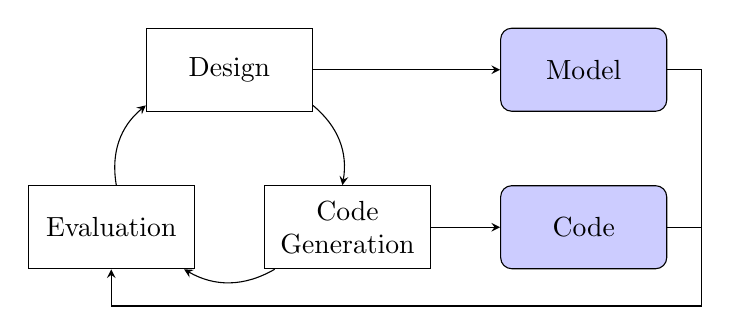
\begin{tikzpicture}[
			node distance = 75, 
			every node/.style={align=center, draw, minimum width=60, minimum height=30},
			>=stealth]
	
		\node(design) at (0,0) {Design};
		\node[rounded corners, fill = blue!20](model) at (4.5,0) {Model};
		\node(generation) at(1.5,-2){Code\\Generation};
		\node[rounded corners, fill = blue!20](code) at (4.5,-2){Code};
		\node(evaluation) at (-1.5,-2) {Evaluation};
	
		\draw[->] (design) -- (model);
		\draw[->] (generation) -- (code);
		
		\draw[->] (design) to[bend left] (generation);
		\draw[->] (generation) to[bend left] (evaluation);
		\draw[->] (evaluation) to[bend left] (design);
		
		\draw[->] (model) -| +(1.5,-3) -| (evaluation);
		\draw (code) -- +(1.5,0);
	\end{tikzpicture}
	}
	
	\smallskip
	
	\pause
	What is our reasoning?
	\begin{itemize}
		\item<+-> Models are easier to check for logical errors
		\item<+-> This also applies to model-model interaction
		\bigskip
		\item<+-> There exists tools to help with model checking
	\end{itemize}
\end{frame}

\section{Model checking}
\subsection{UPPAAL}
\begin{frame}[t]{Model checking}
	\framesubtitle{UPPAAL}
	
	\begin{block}{Description}
		\footnotesize 
		``Uppaal is an integrated tool environment for modeling, 
		validation and verification of real-time systems modeled as networks of timed automata, 
		extended with data types (bounded integers, arrays, etc.).''\footnote{http://www.uppaal.org/}
	\end{block}
	
	\begin{columns}[T]
		\begin{column}{.48\textwidth}
			\begin{itemize}
				\item Represented as automatas
				\item Querys can check for errors
			\end{itemize}
		\end{column}
		\begin{column}{.48\textwidth}
			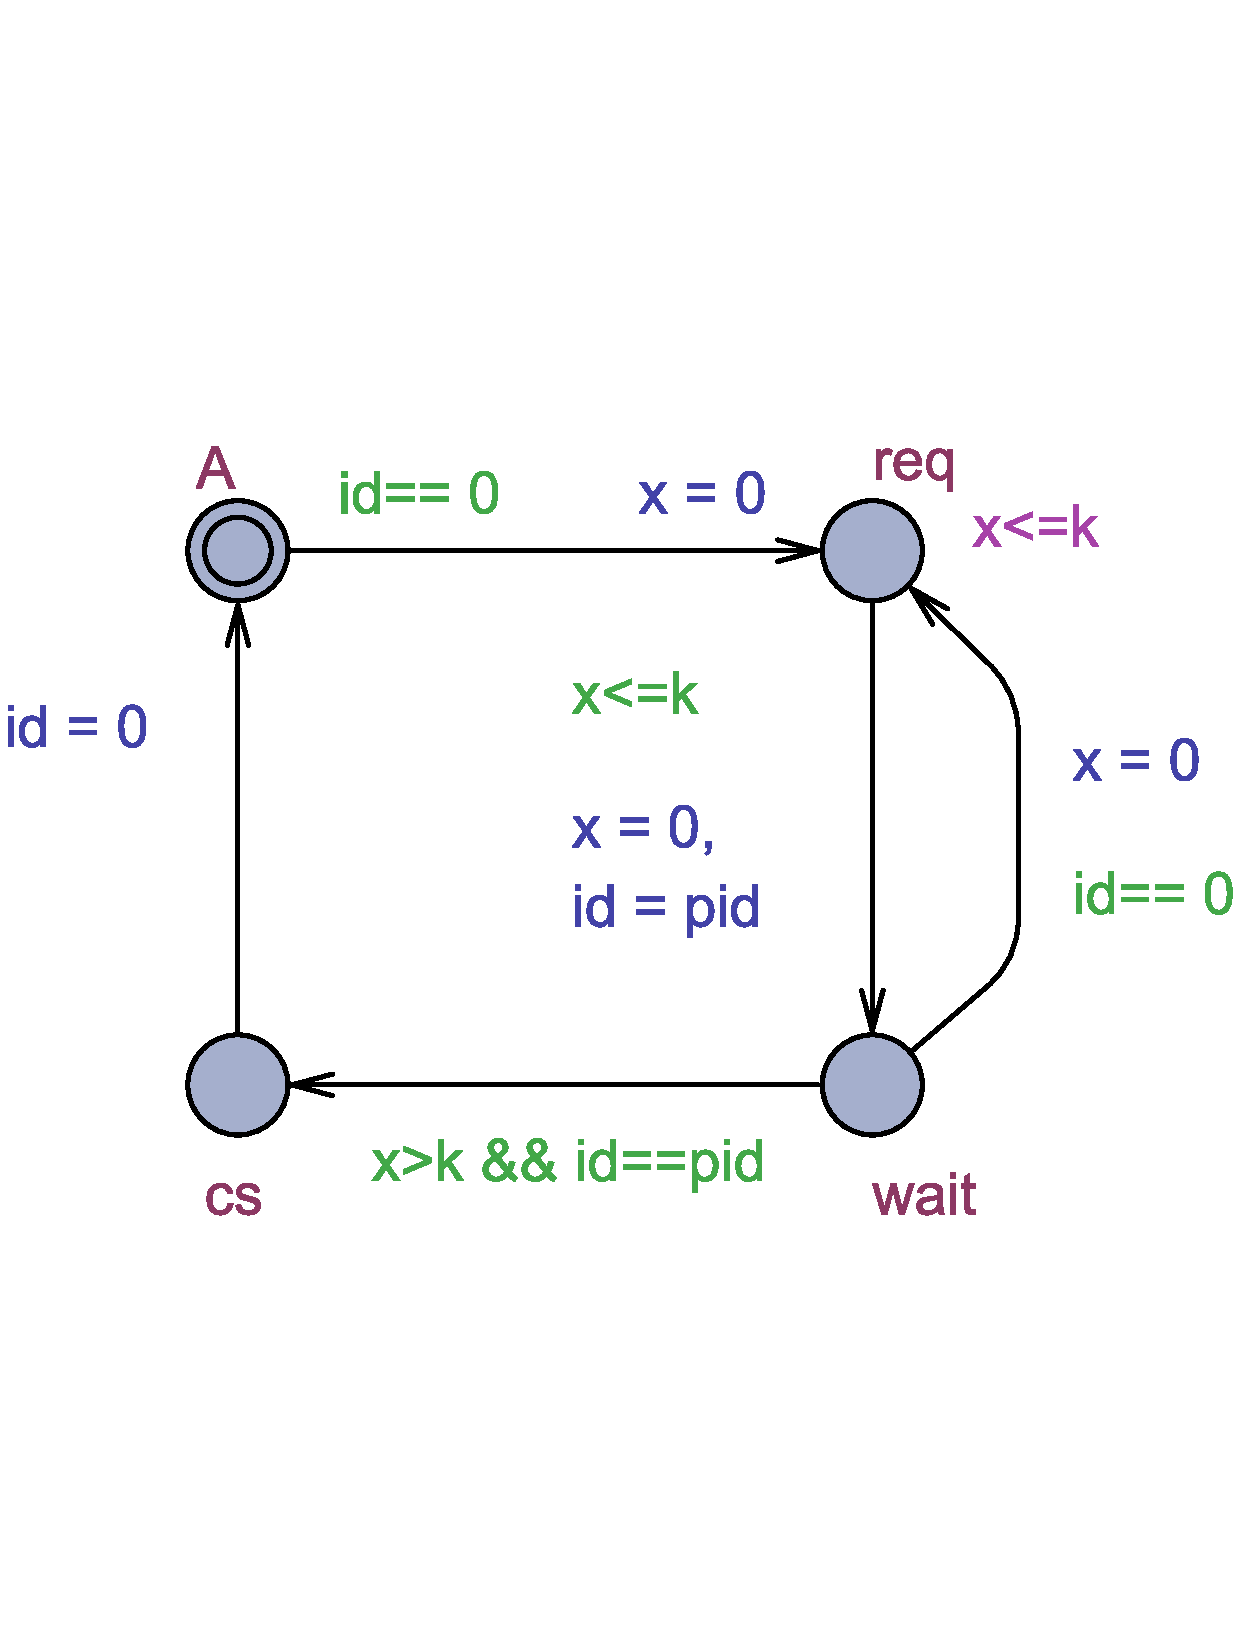
\includegraphics[trim=0 200 0 200,width=0.90\textwidth]{images/P.pdf}
		\end{column}
	\end{columns}
	\medskip
	\texttt{A[] forall (i:id\_t) forall (j:id\_t) P(i).cs \&\& P(j).cs imply i == j}
\end{frame}

\subsection{SMC}
\begin{frame}[t]{Model checking}
	\framesubtitle{Statistical Model Checking (SMC)}
	
	\begin{columns}[T]
		\begin{column}{.48\textwidth}
			Some great thing
			
			\begin{itemize}
				\item<+-> Some properties can not be guarenteed
				\item<+-> What are the chances of those being true?
			\end{itemize}
		\end{column}
		\begin{column}{.48\textwidth}
			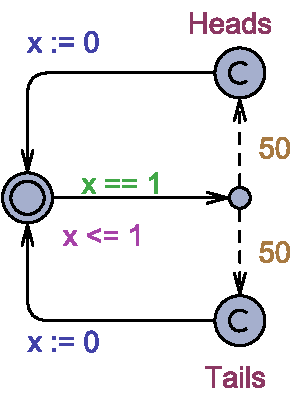
\includegraphics[trim=0 200 0 200,width=0.8\textwidth]{images/Simple_SMC.pdf}
		\end{column}
	\end{columns}
	
	\texttt{Pr[<=300000] (<> exists (i : id\_t) Coin(i).Tails)}
\end{frame}